\subsection{Evaluation}
\label{sec:model_evaluation_description}

In diesem Abschnitt des Modells wird die Operationalisierung der externen Qualität von Erklärungen erläutert. Dabei werden sowohl die Eigenschaften von integrierten Erklärungen an sich beschrieben als auch Effekte, die durch den Einfluss von Erklärbarkeit auf weitere Qualitätsaspekte messbar sind. Dabei werden die schon in \autoref{sec:model_external_dependencies} vorgestellten Qualitätsziele betrachtet.

Es wird von mehreren Autoren festgestellt, dass das Messen der Qualität von Erklärungen aufgrund der stark unterschiedlichen subjektiven Wahrnehmung von \textit{End Usern}  eine Herausforderung darstellt \cite{nunes_systematic_2017, eiband_impact_2019, kouki_user_2017}. Daher werden in vorhandener Literatur zur Evaluation von Erklärungen vor allem subjektive Fragebögen verwendet. Diese orientieren sich in der Regel an den zuvor ausgewählten Zielen für zu integrierende Erklärungen (siehe \autoref{sec:model_external_dependencies}).

Grundsätzlich wird bei der Evaluation zwischen subjektiven Metriken (\textit{qualitative} \cite{wohlin2012experimentation}) und Verhaltensmetriken (\textit{quantitative} \cite{wohlin2012experimentation}) unterschieden. Entsprechend sind die verschiedenen Evaluationsmethoden im Modell in \textit{Qualitative Research} und \textit{Quantitative Research} gegliedert. \citeauthor{waa_evaluating_2021} betonen, dass zur Beurteilung der Qualität von Erklärungen beide Methoden zusammen eingesetzt werden sollten. Sie schreiben, dass es so möglich ist, die \glqq komplette Perspektive\grqq{} auf eine Erklärung zu erhalten \cite[übersetzt vgl.][]{waa_evaluating_2021}.

Auch werden in der Literatur sowohl Studien durchgeführt, bei denen die Teilnehmer jeweils mehrere Bedingungen, wie z.B. verschiedene Erklärungstypen nacheinander evaluieren (\textit{with-in subject}) als auch solche, bei denen pro Teilnehmer nur eine Bedingung evaluiert und diese dann verglichen werden (\textit{between subject}).

Des Weiteren stehen grundsätzlich die von \citeauthor{wohlin2012experimentation} definierten Evaluationsstrategien, die bereits in den Ergebnissen der Literaturrecherche (\autoref{sec:literature_review}) vorgestellt wurden, zum Messen der Qualität von Erklärungen zur Verfügung: \textit{Survey}, \textit{Case Study}, \textit{Experiment}. Diese werden unter anderem von \citeauthor{ribera2019can} sowie \citeauthor{doshi2017towards} auf Erklärbarkeit übertragen. Die verwendete Strategie hängt dabei vom \textit{Context} und den \textit{Objectives} ab. Je nachdem, welche Ergebnisse Stakeholder, die Erklärungen in ein System integrieren möchten, benötigen, muss die Evaluation kontrollierter oder weniger kontrolliert sein. Die Vor- und Nachteile dessen sind bei \citeauthor{wohlin2012experimentation} nachzulesen \cite{wohlin2012experimentation}.

\begin{figure}[htb!]
    \begin{center}
        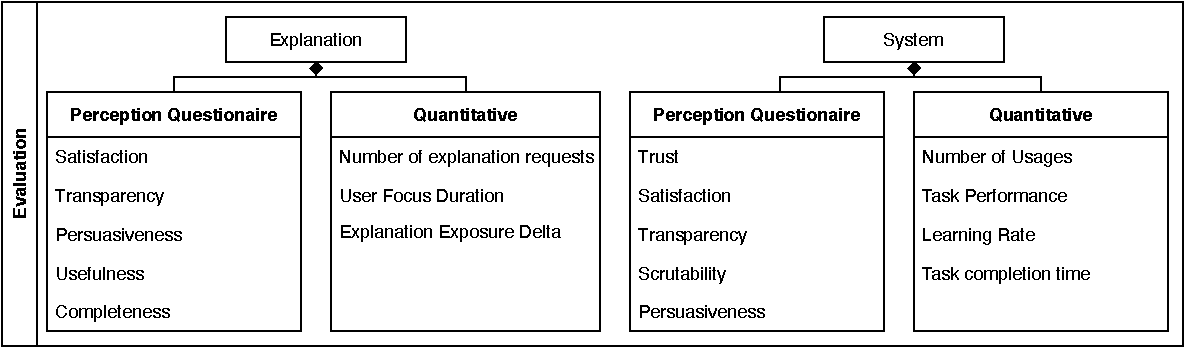
\includegraphics[width=\textwidth]{contents/05_model_description/res/model_evaluation_overview.pdf}
    \end{center}
    \caption{Übersicht über die \textit{Evaluation} von Erklärungen}
    \label{fig:model_evaluation_overview}
\end{figure}

\subsubsection{Qualitative Evaluation}

Bei der qualitativen Evaluation von Erklärungen gibt es verschiedene Möglichkeiten. Entweder wird die Qualität der Erklärungen direkt gemessen. Alternativ wurden in der Literatur aber auch die bereits vorgestellten Qualitätsaspekte (siehe \autoref{sec:model_external_dependencies}) verwendet, um über den Einfluss von Erklärungen auf diese, die externe Qualität von Erklärungen abzuleiten.

Neben den in \autoref{sec:model_external_dependencies} vorgestellten Qualitätsaspekten, die als Qualitätsziele für die Integration von Erklärungen definiert wurden, gibt es weitere Aspekte, die in der Literatur zur Messung der direkten Qualität von Erklärungen vorgestellt wurden \cite{sato_action-triggering_2019}. Diese werden im Folgenden erläutert.

\paragraph{Usefulness} \textit{Usefulness} oder auch \textit{Helpfulnesss} ist der Grad zu dem \textit{End User}, die Erklärungen erhalten, das subjektive Empfinden haben, dass eine Erklärung sie bei der Nutzung oder dem Verständnis über ein System unterstützt haben. 

\paragraph{Completeness} \textit{Completeness} ist das subjektive Empfinden von \textit{End Usern}, dass gegebene Erklärungen einen vollständigen Aufschluss über den erklärten Systembestandteil geben und keine Informationen weglassen.

\bigskip

Bei der subjektiven Evaluation setzt die Literatur vor allem Likert-Skalen ein \cite{sato_action-triggering_2019, sato_context_nodate, wang_is_2018}. Dabei handelt es sich um eine Ordinalskala mit in der Regel fünf oder sieben einzelnen Bewertungsschritten, auf denen eine Aussage bewertet werden kann. In der Regel ist dabei die Zustimmung oder Ablehnung einer Aussage von Interesse. Die genaue Benennung der Bewertungsschritte erfolgt in der Literatur verschieden. Allerdings werden meist solche mit einer inhaltlichen Übereinstimmung zu \glqq Volle Zustimmung\grqq{}, \glqq Teilweise Zustimmung\grqq{}, \glqq Neutral\grqq{},\glqq Teilweise Ablehnung\grqq{} und \glqq Volle Ablehnung\grqq{} verwendet \cite{hoffman_metrics_nodate, koo_understanding_2016, koo_why_2015, hernandez-bocanegra_effects_2020}. Aussagen, welche nicht dem Muster entsprechen, wurden in der folgenden Zusammenfassung in das Format überführt. \autoref{tab:evaluation_qualitative_explanation_measures} und \autoref{tab:evaluation_qualitative_explanation_system_measures} stellen eine Übersicht von verwendeten Aussagen für die Messung der Qualitätsaspekte dar, über welche die Erklärungsqualität messbar ist. Zusammengefasst sind nur verallgemeinerbare Aussagen und nicht solche, die nur einen spezifischen \textit{Context} betreffen.

In spitzen Klammer sind Platzhalter dargestellt, um die aufgelisteten Aussagen besser auf einen \textit{Context} anpassen zu können. \glqq <System>\grqq{} steht entweder für das aktuelle System, Teilsysteme, Tools oder Algorithmen, welche evaluiert werden sollen. \glqq <Erklärung>\grqq{} steht für eine spezifische Erklärung, die evaluiert wird. Die Aufgabe(n), die ein \textit{End User} während einer Evaluation erledigt werden, können im Platzhalter \glqq Aufgabe\grqq{} eingesetzt werden. Darüber werden in eckigen Klammern optionale Teile von Aussagen angegeben, die nur für manche Evaluationskontexte sinnvoll sind.

In \autoref{tab:evaluation_qualitative_explanation_measures} werden die Aussagen zur Evaluation zusammengefasst, die nur für \textit{End User} infrage kommen, die eine Erklärung direkt evaluieren sollen. Die Aussagen beziehen sich dabei direkt auf die Eigenschaften der Erklärung.

\begin{table}[htb!]
    \begin{center}
        \begin{tabular}{p{.3\textwidth}p{.64\textwidth}}
            \hline
            Qualitätsaspekt & Aussage \\
            \toprule
            Satisfaction    & <Erklärung>, stellt mich mit meinem Verständnis über <System> zufrieden.
                                \cite[vgl.][]{riveiro_thats_2021} \\
                            & <Erklärung>, ist zufriedenstellend.
                                \cite[vgl.][]{riveiro_thats_2021, hoffman_metrics_nodate, balog_measuring_2020} \\
            \tablerowspacing
            Perceived Transparency    & Die Informationen der Erklärung waren ausreichend, um <Aufgabe> gut zu erfüllen. 
                                \cite[vgl.][]{wang_is_2018, balog_measuring_2020} \\
            \tablerowspacing
            Persuasiveness  & <Erklärung>, ist überzeugend.
                                \cite[vgl.][]{sato_action-triggering_2019, sato_context_nodate} \\
                            & <Erklärung>, weckt Interesse. 
                                \cite[vgl.][]{sato_action-triggering_2019, sato_context_nodate} \\
            \tablerowspacing
            Usefulness      & <Erklärung>, ist einfach zu verstehen. 
                                \cite[vgl.][]{sato_action-triggering_2019, sato_context_nodate} \\
                            & <Erklärung>, ist nützlich bei der Erfüllung von <Aufgabe>.
                                \cite[vgl.][]{sato_action-triggering_2019, sato_context_nodate, hoffman_metrics_nodate, balog_measuring_2020} \\
            \tablerowspacing
            Completeness    & <Erklärung>, ist hinreichend vollständig.
                                \cite[vgl.][]{hoffman_metrics_nodate, riveiro_thats_2021} \\
                            & <Erklärung>, ist hinreichend detailliert.
                                \cite[vgl.][]{riveiro_thats_2021} \\
            \toprule
        \end{tabular}
    \end{center}
    \caption{Aussagen zur qualitativen Evaluation ausgewählter externer Qualitätsaspekte in Bezug auf Erklärungen in einem System}
    \label{tab:evaluation_qualitative_explanation_measures}
\end{table}

In der Übersicht, die in \autoref{tab:evaluation_qualitative_explanation_system_measures} zu sehen ist, werden Aussagen zusammengefasst, welche auf beide der zuvor erwähnten Situationen anpassbar sind. Je nachdem, ob die aktuelle Messung sich direkt auf eine Erklärung bezieht, müssen die optionalen Teile dabei weggelassen werden. Wenn alle optionalen Teile eingefügt werden, ist es bei \textit{within-subject} Studien möglich, einen Vergleich zwischen verschiedenen Bedingungen zu ziehen, da die Teilnehmer eine Präferenz angeben können.

\begin{table}[htb!]
    \begin{center}
        \begin{tabular}{p{.3\textwidth}p{.64\textwidth}}
            \hline
            Qualitätsaspekt & Aussage \\
            \toprule
            % \hline
            % Effectivity     & Ich konnte <Aufgabe> [mithilfe von <Erklärung>] erfolgreich[er] erledigen.
            %                     \cite[vgl.][]{balog_measuring_2020, hernandez-bocanegra_effects_2020} \\
            % \hline
            % Efficiency      & Ich konnte <Aufgabe> [mithilfe von <Erklärung>] schnell[er] erledigen.
            %                     \cite[vgl.][]{balog_measuring_2020, hernandez-bocanegra_effects_2020} \\
            Trust           & Ich kann [mithilfe von <Erklärung>] [besser] sagen, wie vertrauenswürdig das System ist.
                                \cite[vgl.][]{hoffman_metrics_nodate, balog_measuring_2020, weitz_you_2019, hernandez-bocanegra_effects_2020} \\
            \tablerowspacing
            Satisfaction    & Ich bin mit der Nutzung von <System> zufrieden[er, mithilfe von <Erklärung>].
                                \cite[vgl.][]{balog_measuring_2020} \\
                            & Ich werde <System> [wegen <Erklärung>] wieder benutzen.
                                \cite[vgl.][]{balog_measuring_2020} \\
            \tablerowspacing
            Transparency    & Ich kann den Entscheidungsprozess von <System> [mithilfe von <Erklärung>] [besser]
                                verstehen.
                                \cite[vgl.][]{wang_is_2018, balog_measuring_2020} \\
                            & Ich kann [mithilfe von <Erklärung>] [besser] verstehen, wie <System> funktioniert.
                                \cite[vgl.][]{riveiro_thats_2021, hoffman_metrics_nodate, hernandez-bocanegra_effects_2020} \\
            \tablerowspacing
            Scrutability    &  Ich kann [mithilfe von <Erklärung>] [besser] sagen, wie zuverlässig <System> ist.
                                \cite[vgl.][]{hoffman_metrics_nodate, balog_measuring_2020} \\
            \tablerowspacing
            Persuasiveness  & Ich bin von den Entscheidungen von <System> [mithilfe von <Erklärung>] überzeugt.
                                \cite[vgl.][]{tsai_effects_2020} \\
            \toprule
        \end{tabular}
    \end{center}
    \caption{Aussagen zur qualitativen Evaluation ausgewählter Qualitätsaspekte in Bezug auf ein System oder Systemteile}
    % Optional können sich die Aussagen auf \textit{End Usern} präsentierte Erklärungen beziehen oder verschiedene Studienbedingungen vergleichen.
    \label{tab:evaluation_qualitative_explanation_system_measures}
\end{table}

Die Aussagen aus \autoref{tab:evaluation_qualitative_explanation_system_measures} können darüber hinaus zum Teil auch als Entscheidungsfragen formuliert werden. Wenn dies der Fall war, wurde in der Literatur für eine der beiden Antwortmöglichkeiten zusätzlich ein Freitextfeld für eine Begründung bereitgestellt, z.~B. \glqq Hätten Sie sich gewünscht, dass die Erklärungen zusätzliche Informationen enthalten? Wenn ja, welche Art von Informationen und wann, d.~h. in welchen Situationen?\grqq \cite[übersetzt vgl.][]{riveiro_thats_2021}.

Als Alternative zu den vorgestellten Aussagen haben außerdem einige Autoren direkt die Präferenz zwischen verschiedenen Formen von Erklärungen abgefragt, statt diese indirekt über Aussagen zu ermitteln \cite{kouki_user_2017, mucha_interfaces_2021, abdulrahman_belief-based_2019, balog_measuring_2020, wiegand_id_2020, stange_effects_2021, kaptein_personalised_2017}.

Des Weiteren gibt es mehrere Beispiele dafür, dass Autoren bei der Messung der Qualität auch den \textit{Mental Workload} von \textit{End Usern} bei der Erfüllung von Aufgaben gemessen haben. Dabei wird überprüft, wie sehr die kognitiven Fähigkeiten der Probanden gefordert werden. Alle betrachteten Beispiele aus der Literatur verwenden dabei den standardisierten Fragebogen \glqq NASA TLX\grqq{} \cite{wiegand2019drive, wiegand_id_2020,du2019look}.

% TODO: Check which aspects should really be evaluated.

Über die bereits vorgestellten Möglichkeiten zur qualitativen Evaluation von Erklärungen untersuchen außerdem mehrere Autoren den Einfluss von Erklärungen auf \textit{Usability}. \textit{Usability} ist dabei definiert als der \glqq Grad, in dem ein Produkt oder System von bestimmten Nutzern verwendet werden kann, um bestimmte Ziele mit \textit{Efficiency}, \textit{Effectivity} und \textit{Satisfaction} in einem bestimmten \textit{Context} zu erreichen \grqq{} \cite[übersetzt vgl.][]{international2011iso}. Die Beispiele aus dem Bereich der Erklärbarkeit fokussieren sich dabei auf die Verwendung von \textit{Think-Aloud}-Studien, bei denen die Studienteilnehmer während der Nutzung eines Systems ihre Gedanken laut aussprechen und sich so \textit{Usability}-Probleme erfassen lassen \cite{wiegand_id_2020, yamada_evaluating_2016}. Hintergrund ist, dass \textit{Explainability} auch negative Effekte auf \textit{Usability} haben kann \cite{chazette_knowledge_nodate} und dies daher auch gemessen werden sollte.

\bigskip

Die zuvor erläuterten qualitativen Metriken zur Messung der Qualität von Erklärungen sind der erste Teil der Antwort dieses Modells auf \textbf{RQ3}. Dabei kann an dieser Stelle zusammengefasst werden, dass der qualitative Teil der Evaluationen von Erklärungen den Großteil der in der Literatur bereits erfolgten Evaluationsmethoden ausmacht und dort aufgrund der stark subjektiven Wahrnehmung von Erklärungen als notwendiger Teil erachtet wird.

\subsubsection{Quantitative Evaluation von Erklärungen}

Die quantitative Messung der Qualität von Erklärungen kommt in der Literatur seltener vor, als die qualitative. Dies liegt unter anderem an dem starken Einfluss der subjektiven Meinungen von \textit{End Usern} in Bezug auf den Bedarf für Erklärungen und dessen Granularität \cite{chazette_end-users_nodate, kouki_user_2017}. Nichtsdestotrotz wird in der Literatur empfohlen zusätzlich auch eine quantitative Evaluation durchzuführen \cite{balog_measuring_2020}. Beispielsweise kommen \citeauthor{wiegand2019drive} zu dem Ergebnis, dass \textit{End User} subjektiv andere Erklärungen präferieren können, als zu einer besseren Performanz der Aufgabenerfüllung der \textit{End User} führen würden \cite{wiegand2019drive}.

Bei direkter Messung von quantitativen Aspekten von Erklärungen wurden in der Literatur neben domänen- oder erklärungs-spezifischen Metriken, solche eingesetzt, die unmittelbar den Bedarf und die Granularität messen. In \autoref{tab:evaluation_quantitative_explanation_measures} sind die Metriken aufgeführt, welche Kontext- und erklärungsunabhängig verallgemeinerbar sind.

\begin{table}[htb!]
    \centering
    \begin{tabular}{p{.2\textwidth}p{.41\textwidth}p{.3\textwidth}}
        \hline
        Aspekt & Metrik & Quellen \\
        \toprule
        Bedarf          & \textit{Number of explanation requests}
            & \cite{wiegand_id_2020} \cite{ chazette_end-users_nodate} \cite{balog_measuring_2020} \\
        \tablerowspacing
        Granularität    & \textit{User Focus Duration} & \cite{balog_measuring_2020} \\
                        & \textit{Explanation Exposure Delta} & \cite{nunes_systematic_2017}\\
        \toprule
    \end{tabular}
    \caption{Quantitative Evaluationsmöglichkeiten zu direkten Messung der Qualität von Erklärungen}
    \label{tab:evaluation_quantitative_explanation_measures}
\end{table}

Wenn eine Erklärung optional angefordert werden kann, ist eine mögliche Metrik zu messen, wie häufig \textit{End User} die Erklärung anfordern (\textit{Number of explanation requests}). Daraus kann abgeleitet werden, wie groß der Bedarf für eine Erklärung in der spezifischen Situation wirklich ist \cite{wiegand_id_2020}.

% Dies lässt sich auch bereits als Gedankenexperiment zuvor bestimmen \cite[vgl.][]{chazette_end-users_nodate}.

Auch kann nach der Anforderung einer Erklärung durch einen \textit{End User} gemessen werden, wie lange dieser sich auf diese fokussiert (\textit{User Focus Duration}) \cite{balog_measuring_2020}. Daraus kann abgeleitet werden, ob die Granularität der Erklärung für den \textit{End User} passend war. Eine weitere Möglichkeit, die Granularität zu messen ist außerdem das \textit{Explanation Exposure Delta} \cite{nunes_systematic_2017}. Hierfür wird eine Metrik zum Verständnis des Systems benötigt, welche auf eine Intervallskala abbildet. Die verwendeten Metriken sind dabei sehr Domänen- und Aufgaben-spezifisch. Diese Metrik wird im Anschluss einmal vor und einmal nach der Anzeige einer Erklärung gemessen. Die Differenz dieser Werte ist das \textit{Explanation Exposure Delta}. Umso größer dies ist, umso mehr Wissen haben \textit{End User} durch eine Erklärung erlangt.

Neben der direkten Evaluation der Eigenschaften von Erklärungen haben deutlich mehr Autoren die Auswirkungen von Erklärungen auf bestimmte Qualitätsaspekte von Systemen untersucht. Im Folgenden werden dabei Metriken vorgestellt, welche in der Literatur verwendet wurden. Auch bei der quantitativen Messung der unter \autoref{sec:model_external_dependencies} vorgestellten externen Qualitätsaspekte, auf die der Einfluss von Erklärungen in der Literatur evaluiert wurde, gibt es über die hier erwähnten hinaus weitere Metriken, welche sich eigenen können. \citeauthor{carvalho2017quality} stellen in ihrer Veröffentlichung eine Übersicht über verschiedene Metriken vor, um u.~a. die in dieser Arbeit erwähnten Qualitätsaspekte zu messen \cite{carvalho2017quality}.

\autoref{tab:evaluation_quantitative_explanation_measures_indirect} fasst die in der Literatur im Bezug auf Erlkärbarkeit genutzten Metriken zusammen. Dabei ist für den Qualitätsaspekt \textit{Trust} die Anzahl der Nutzungen (\textit{Number of Usages}) aufgeführt. Diese kann sowohl absolut als auch relativ zu einem Zeitraum betrachtet werden. Die \textit{Task Performance} ist hier als abstrakte Metrik aufgeführt. Unter diesem Begriff haben mehrere Autoren jeweils die Qualität der Aufgabenausführung von \textit{End Usern} zusammengefasst. Konkrete Metriken werden hier allerdings nicht aufgeführt, da diese laut mehrerer Autoren sehr \textit{Context}-abhängig sind \cite{tintarev2007survey, gunning2019darpa}. Die \textit{Task Performance} wird dabei sowohl für die Bewertung der \textit{Persuasiveness} des Systems als auch die \textit{Efficiency} herangezogen. Für letztere haben \citeauthor{tintarev_designing_nodate} sowie \citeauthor{gunning2019darpa} außerdem die \textit{Learning Rate} als Evaluationsfaktor herangezogen. Sie vergleichen dabei unter verschiedenen Bedingungen, wie schnell sich die \textit{Task Performance} von \textit{End Usern} erhöht.

\begin{table}[htb!]
    \begin{center}
        \begin{tabular}{p{.25\textwidth} p{.25\textwidth} p{.4\textwidth}}
            \hline
            Qualitätsaspekt & Metrik & Quellen \\
            \toprule
            Trust           & \textit{Number of Usages} & \cite{tintarev2007survey} \\
            \tablerowspacing
            Persuasiveness  & \textit{Task Performance} & \cite{tintarev2007survey} \\
            \tablerowspacing
            Effectiveness   & \textit{Task Performance} &
                                \cite{waa_evaluating_2021} \cite{mucha_interfaces_2021}
                                \cite{tintarev_designing_nodate} \cite{abdulrahman_belief-based_2019}
                                \cite{zolotas_towards_2019} \cite{martin_developing_2019} \cite{martin_evaluating_2021}
                                \cite{gunning2019darpa} \cite{kunkel_let_2019} \cite{tintarev2007survey} \\
                            & \textit{Learning Rate}    &
                                \cite{tintarev_designing_nodate} \cite{gunning2019darpa} \\
            \tablerowspacing
            Efficiency & \textit{Task Completion Time} & \cite{tintarev2007survey} \\
            \toprule
        \end{tabular}
    \end{center}
    \caption{Evaluation}
    \label{tab:evaluation_quantitative_explanation_measures_indirect}
\end{table}

\noindent\fbox{
    \parbox{0.964\textwidth}{
        \smallskip
        \textbf{RQ3} Auf welche Art und Weise kann evaluiert werden, ob die in ein erklärbares System integrierten Erklärungen das Ziel der Integration bezogen auf externe Qualitätsaspekte erfüllt haben?
        \smallskip
    }
}

\smallskip

Der Abschnitt \textit{Evaluation} des Modells für Erklärungen ist die Antwort auf die dritte Forschungsfrage. Die Antwort auf die Frage nach der Evaluation von Erklärungen ist dabei drei geteilt. Zunächst enthält das Modell einen kurzen Überblick über das Studiendesign für verschiedene Anwendungsfälle. Außerdem sind Teil der Antwort die zwei verschiedene Evaluationsmöglichkeiten: direkte Erklärungsevaluation und Evaluation der Auswirkungen auf das System im Allgemeinen. Für beide Varianten bietet das Modell dabei Beispiele für qualitative und quantitative Betrachtungen. Dies erfüllt auch die Anforderung an den Leitfaden ([GR3])

Als klares Fazit muss des Weiteren gezogen werden, dass für eine ganzheitliches Bild über die Qualität von Erklärungen sowohl qualitativ als auch quantitativ die Erklärungen an sich sowie dessen Auswirkung auf weitere externe Qualitätsaspekte betrachtet werden müssen \cite{balog_measuring_2020}. Wichtig ist dabei auch die Betrachtung von Aspekten zur Kontrolle, auf die ggf. negative Effekte durch Erklärungen möglich sind.

\bigskip

Nachdem das in den vorigen Abschnitten vorgestellte Modell die Forschungsfragen \textbf{RQ1} - \textbf{RQ3} beantwortet fehlt nun eine Zusammenfassung der Abhängigkeiten der einzelnen Aspekte des Modells. Neben der Beantwortung der Forschungsfragen \textbf{RQ4.1} und \textbf{RQ4.2} ist dies beispielsweise auch von nöten, um festzulegen, welche Qualitätsaspekte bei der Evaluation von Erklärungen betrachtet werden müssen.